% -- raw data
%     describe the dataset, total # of participants in each group before and after dataset cleaning, demographics of each group;
%(To-do: maybe add a hierarchical graph the represents how responses from different paths are aggregated)
    % mode=text
% donation descriptive statistics: perc of non-zero donation, total donation amount comparison across groups, donation distribution across topics between groups
% The donation rate in each condition closely centered around the average donation rate, ranging from $70.37\%$ (in QV108) and $77.19\%$ (in Likert).
% Aggregated across all participants,
% the amount of donations for each 
% of the nine charities have a similar trend
% shown in Figure \ref{fig:topic_don_exp1}. 
% Environment-related, health-related, and human-related charities 
% were consistently the more popular 
% compared to the art-related, international-related, and faith-related charities.
% However, there are some differences 
% when observing the population-level preferences 
% towards charities across the four surveying methods. 
% For example, the pets-related charity 
% received far less donation in percentage 
% for the Likert Group compared with the QV groups. 
% This suggests that there was a good amount of variance 
% in people's opinions toward the nine topics, 
% making the surveying task meaningful.
% \begin{figure}[htpb]
%     \centering
%     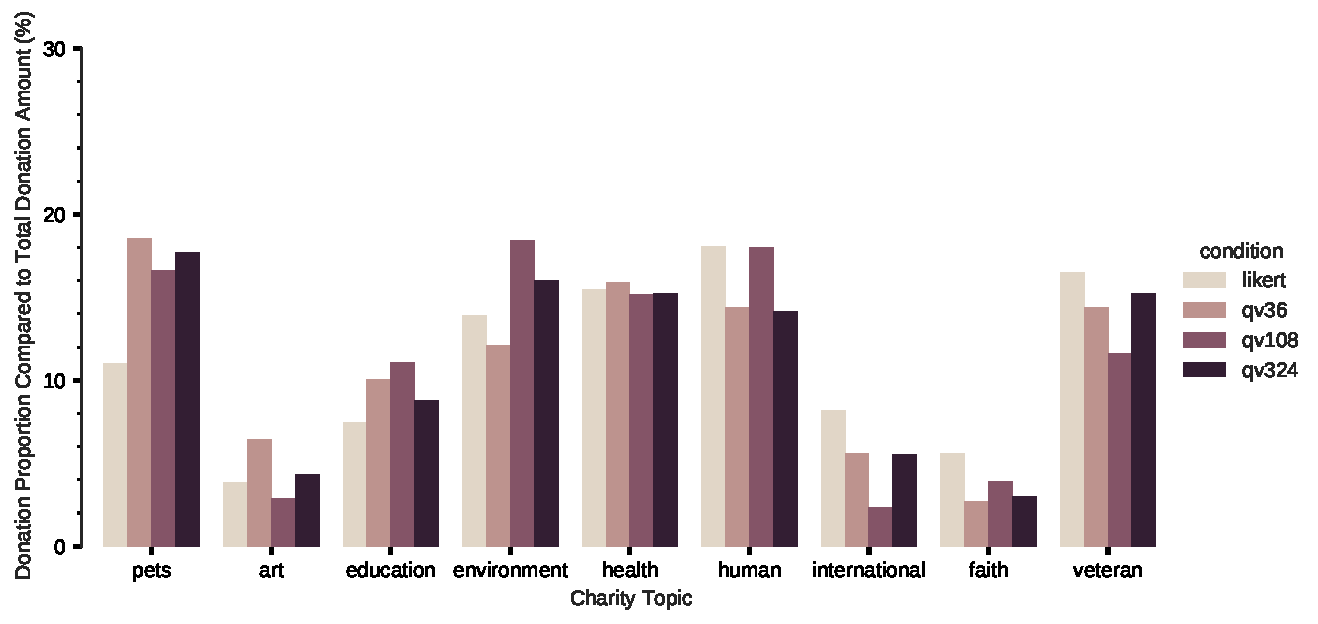
\includegraphics[width=\textwidth, keepaspectratio=true]{content/image/normalized_contributions_per_topic_across_conditions.pdf}
%     \caption{
%       Percentage Contribution Amount per Topic with Respect to the Total Donation Amount across Conditions.
%       We see a general trend of the more and less popular charities while some differences across each
%       surveying method within each group.
%     }
%     \Description[Percentage Contribution Amount per Topic with Respect to the Total Donation Amount across Conditions for experiment 1]{
%       Percentage Contribution Amount per Topic with Respect to the Total Donation Amount across Conditions.
%       We see a general trend of the more and less popular charities while some differences across each
%       surveying method within each group.
%     }
%     \label{fig:topic_don_exp1}
% \end{figure}
%     QV & Likert votes descriptive statistics: votes distribution per topic across groups, budget usage distribution across QV groups
% The sufficient amount of variations shown across topics indicated that our prompt in the experiment, which we reminded participants that resources are limited and one should express their relative preferences worked as intended. 
% but the tail of lower percentage usage in QV324 was longer then in the other two cases. 
% mention the implication of longer tail in QV324 in the discussion section: 
% need to be aware of using an overly large budget and resulting in a worse tail
% Visualize the raw voting and donation data together to show covariation
% To check if the fitted distributions described the data well, please refer to the discussion about posterior predictive check in 
% The posterior distributions of the scale parameter $\sigma$ in all four likelihood functions are similar, with a mode ranging from $13.904$ and $15.724$.
% The posterior of the pooled QV condition is simply the averages of the values of the posteriors from QV36, QV108 and QV324 for every step in the MCMC, because the MCMC jointly estimates the posteriors of all variables at every step. 
% Similiar claim that QV allows better alignment to ones true preference
% can be supported by Qualitative Analysis Results.
% We ask participants to provide a freeform text response on the reason why they made the choices they made
% when participants filled out the Likert survey or QV survey,
% Of all surveys ($N=394$) across both groups, most participants filled out the surveys ($N=331$) based on what they think are the most important issues to them. %84 percent
% Besides, a small portion of participants ($N=30$) used their instincts when replying to the survey.
% Some participants either think that every aspect is important ($N=7$) or that resources should be equally distributed ($N=7$). 